\documentclass{article}
\usepackage{amsmath}
\usepackage{graphicx}
\graphicspath{images}
\usepackage{hyperref}


\title{World of FineCraft}
\author{Susanne Gjersund}
\date{18.10.2018}
\makeindex

\begin{document}
	
	
	\maketitle
	\newpage
	\maketitle
	\tableofcontents
	\newpage


\section{Introduction}
	





\section{The different Sorting Algorithms}


\subsection{Merge Sort}


\textbf{Worst-Case performance}\\ 
$O(n\log n)$ \\
\textbf{Best-Case performance}\\ 
$O(n\log n)$ \\
\textbf{Average performance}\\ 
$O(n\log n)$ \\


Time complexity of Merge Sort is $\theta(n\log n)$ in all 3 cases (worst, average and best) as merge sort always divides the array in two halves and take linear time to merge two halves.


Applications of Merge Sort

Merge Sort is useful for sorting linked lists in O(nLogn) time.In case of linked lists the case is different mainly due to difference in memory allocation of arrays and linked lists. Unlike arrays, linked list nodes may not be adjacent in memory. Unlike array, in linked list, we can insert items in the middle in O(1) extra space and O(1) time. Therefore merge operation of merge sort can be implemented without extra space for linked lists.
In arrays, we can do random access as elements are continuous in memory. Let us say we have an integer (4-byte) array A and let the address of A[0] be x then to access A[i], we can directly access the memory at (x + i*4). Unlike arrays, we can not do random access in linked list. Quick Sort requires a lot of this kind of access. In linked list to access i’th index, we have to travel each and every node from the head to i’th node as we don’t have continuous block of memory. Therefore, the overhead increases for quick sort. Merge sort accesses data sequentially and the need of random access is low.

Inversion Count Problem
Used in External Sorting

\begin{figure}[h]
	\centering
	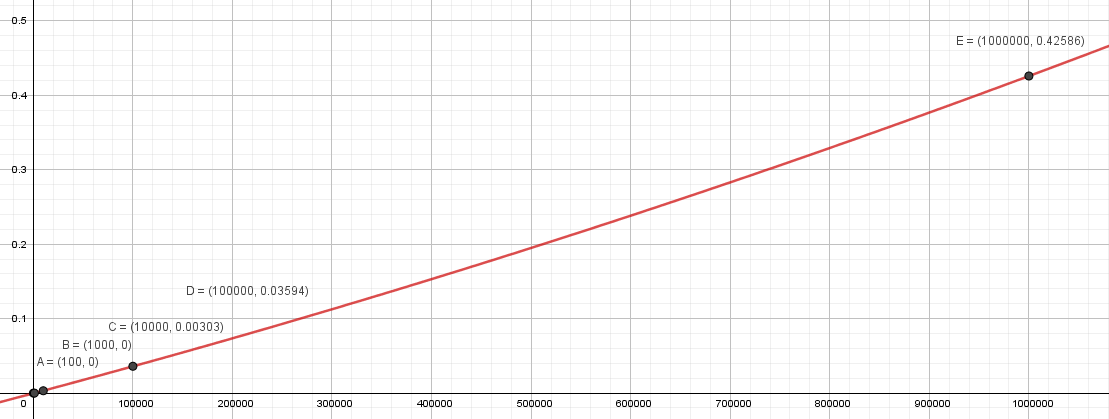
\includegraphics[width=0.7\linewidth]{images/mergeSort}
	\caption{Merge Sort performance}
	\label{fig:mergesort}
\end{figure}












\subsection{Insertion Sort}

Insertion Sort
Insertion sort is a simple sorting algorithm that works the way we sort playing cards in our hands.
Algorithm
// Sort an arr[] of size n
insertionSort(arr, n)
Loop from i = 1 to n-1.
……a) Pick element arr[i] and insert it into sorted sequence arr[0…i-1]


Another Example: 
12, 11, 13, 5, 6

Let us loop for i = 1 (second element of the array) to 5 (Size of input array)

i = 1. Since 11 is smaller than 12, move 12 and insert 11 before 12
11, 12, 13, 5, 6

i = 2. 13 will remain at its position as all elements in A[0..I-1] are smaller than 13
11, 12, 13, 5, 6

i = 3. 5 will move to the beginning and all other elements from 11 to 13 will move one position ahead of their current position.
5, 11, 12, 13, 6

i = 4. 6 will move to position after 5, and elements from 11 to 13 will move one position ahead of their current position.
5, 6, 11, 12, 13


Time Complexity: O(n*2)

Auxiliary Space: O(1)

Boundary Cases: Insertion sort takes maximum time to sort if elements are sorted in reverse order. And it takes minimum time (Order of n) when elements are already sorted.

Algorithmic Paradigm: Incremental Approach

Sorting In Place: Yes

Stable: Yes

Online: Yes

Uses: Insertion sort is used when number of elements is small. It can also be useful when input array is almost sorted, only few elements are misplaced in complete big array.

What is Binary Insertion Sort?
We can use binary search to reduce the number of comparisons in normal insertion sort. Binary Insertion Sort find use binary search to find the proper location to insert the selected item at each iteration. In normal insertion, sort it takes O(i) (at ith iteration) in worst case. we can reduce it to O(logi) by using binary search. The algorithm as a whole still has a running worst case running time of O(n2) because of the series of swaps required for each insertion. Refer this for implementation.

How to implement Insertion Sort for Linked List?
Below is simple insertion sort algorithm for linked list.

1) Create an empty sorted (or result) list
2) Traverse the given list, do following for every node.
......a) Insert current node in sorted way in sorted or result list.
3) Change head of given linked list to head of sorted (or result) list. 


\subsection{Selection Sort}

Selection Sort
The selection sort algorithm sorts an array by repeatedly finding the minimum element (considering ascending order) from unsorted part and putting it at the beginning. The algorithm maintains two subarrays in a given array.

1) The subarray which is already sorted.
2) Remaining subarray which is unsorted.

In every iteration of selection sort, the minimum element (considering ascending order) from the unsorted subarray is picked and moved to the sorted subarray.

Following example explains the above steps:


Time Complexity: O(n2) as there are two nested loops.

Auxiliary Space: O(1)
The good thing about selection sort is it never makes more than O(n) swaps and can be useful when memory write is a costly operation.

Exercise : 
Sort an array of strings using Selection Sort

Stability : The default implementation is not stable. However it can be made stable. Please see stable selection sort for details.

In Place : Yest, it does not require extra space.







\subsection{Quick Sort}








\subsection{Binary Search Tree}

Binary Search Tree is a node-based binary tree data structure which has the following properties:

The left subtree of a node contains only nodes with keys lesser than the node’s key.
The right subtree of a node contains only nodes with keys greater than the node’s key.
The left and right subtree each must also be a binary search tree.








\subsection{Heap Sort}

Heap sort is a comparison based sorting technique based on Binary Heap data structure. It is similar to selection sort where we first find the maximum element and place the maximum element at the end. We repeat the same process for remaining element.

What is Binary Heap?
Let us first define a Complete Binary Tree. A complete binary tree is a binary tree in which every level, except possibly the last, is completely filled, and all nodes are as far left as possible (Source Wikipedia)

A Binary Heap is a Complete Binary Tree where items are stored in a special order such that value in a parent node is greater(or smaller) than the values in its two children nodes. The former is called as max heap and the latter is called min heap. The heap can be represented by binary tree or array.



Why array based representation for Binary Heap?
Since a Binary Heap is a Complete Binary Tree, it can be easily represented as array and array based representation is space efficient. If the parent node is stored at index I, the left child can be calculated by 2 * I + 1 and right child by 2 * I + 2 (assuming the indexing starts at 0).

Heap Sort Algorithm for sorting in increasing order:
1. Build a max heap from the input data.
2. At this point, the largest item is stored at the root of the heap. Replace it with the last item of the heap followed by reducing the size of heap by 1. Finally, heapify the root of tree.
3. Repeat above steps while size of heap is greater than 1.

How to build the heap?
Heapify procedure can be applied to a node only if its children nodes are heapified. So the heapification must be performed in the bottom up order.



Notes:
Heap sort is an in-place algorithm.
Its typical implementation is not stable, but can be made stable (See this)

Time Complexity: Time complexity of heapify is $O(\log n)$. Time complexity of createAndBuildHeap() is $O(n)$ and overall time complexity of Heap Sort is $O(n\log n).$

Applications of HeapSort
1. Sort a nearly sorted (or K sorted) array
2. k largest(or smallest) elements in an array

Heap sort algorithm has limited uses because Quicksort and Mergesort are better in practice. Nevertheless, the Heap data structure itself is enormously used. See Applications of Heap Data Structure



\subsection{std::Sort}

Sorting is one of the most basic functions applied to data. It means arranging the data in a particular fashion, which can be increasing or decreasing. There is a built-in function in C++ STL by the name of sort().

std::sort() is a generic function in C++ Standard Library, for doing comparison sorting.


Time Complexity
Best Case – O(N log N)
Average Case- O(N log N)
Worse Case- O(N log N)
where, N = number of elements to be sorted.

Algorithms used by sort()
The algorithm used by sort() is IntroSort. Introsort being a hybrid sorting algorithm uses three sorting algorithm to minimise the running time, Quicksort, Heapsort and Insertion Sort. Simply putting, it is the best sorting algorithm around. It is a hybrid sorting algorithm, which means that it uses more than one sorting algorithms as a routine.




\section{Comparing Algorithms}


\end{document}